%\chapter{Limits of Random Variables}


\chapter{Limit Laws of Statistics}\label{S:LimitLawsStats}

\section{Convergence of Random Variables}\label{S:ConvOfRVs}

This important topic is concerned with the limiting behavior of sequences of RVs. 
We want to understand what it means for a sequence of random variables $\{X_n\}_{n=1}^{\infty} := X_1,X_2,\ldots$ to converge to another random variable $X$, when all RVs are defined on the same probability space $(\Omega,\mathcal{F},\p)$.
\[
\{X_i \}_{i=1}^n := X_1,X_2,X_3, \ldots X_{n-1}, X_n \qquad \text{as  $n \rightarrow \infty$ .}
\]
From a statistical or decision-making viewpoint, as you will see in Inference Theory I course, $n \rightarrow \infty$ is associated with the amount of data or information $\rightarrow \infty$.  
More abstractly, we are interested in what happens to the limiting RV $X := \lim_{n\to \infty} X_n$ when given the DFs $F_n(x)$ for each $X_n$. 

We need different notions of convergence to characterize such a behavior: two simplest behaviors are that the sequence eventually takes a constant value $\theta$, 
i.e. $X_n$ approaches $X \sim \pointmass(\theta)$ RV, or that values in the sequence continue to change but can be described by an unchanging probability distribution, i.e., $X_n$ approaches $X \sim F(x)$. See \url{https://en.wikipedia.org/wiki/Convergence_of_random_variables}.

Let us first refresh ourselves with notions of convergence, limits and continuity in the real line (\hyperref[S:AnalysisRefresher]{Sec.~\ref*{S:AnalysisRefresher}}) before proceeding further.

Can the sequences of $\{\pointmass(\theta_i=17)\}_{i=1}^{\infty}$ and $\{\pointmass(\theta_i=1/i)\}_{i=1}^{\infty}$ RVs be the same as the two sequences of real numbers $\{ x_i \}_{i=1}^{\infty} = 17, 17, 17, \ldots$ and $\{ x_i \}_{i=1}^{\infty} = \frac{1}{1},\frac{1}{2},\frac{1}{3}, \ldots$ we saw in Examples~\ref{EX:limOf17s} and \ref{EX:limin1overi}?


Yes why not -- just move to space of distributions over the reals! See Figure~\ref{F:SequenceOfPointMassRVS17And1Byi}.

\begin{figure}[htpb]
\caption{Sequence of $\{\pointmass(17)\}_{i=1}^{\infty}$ RVs (left panel) and $\{\pointmass(1/i)\}_{i=1}^{\infty}$ RVs (only the first seven are shown on right panel) and their limiting RVs in red.\label{F:SequenceOfPointMassRVS17And1Byi}}
\centering   \makebox{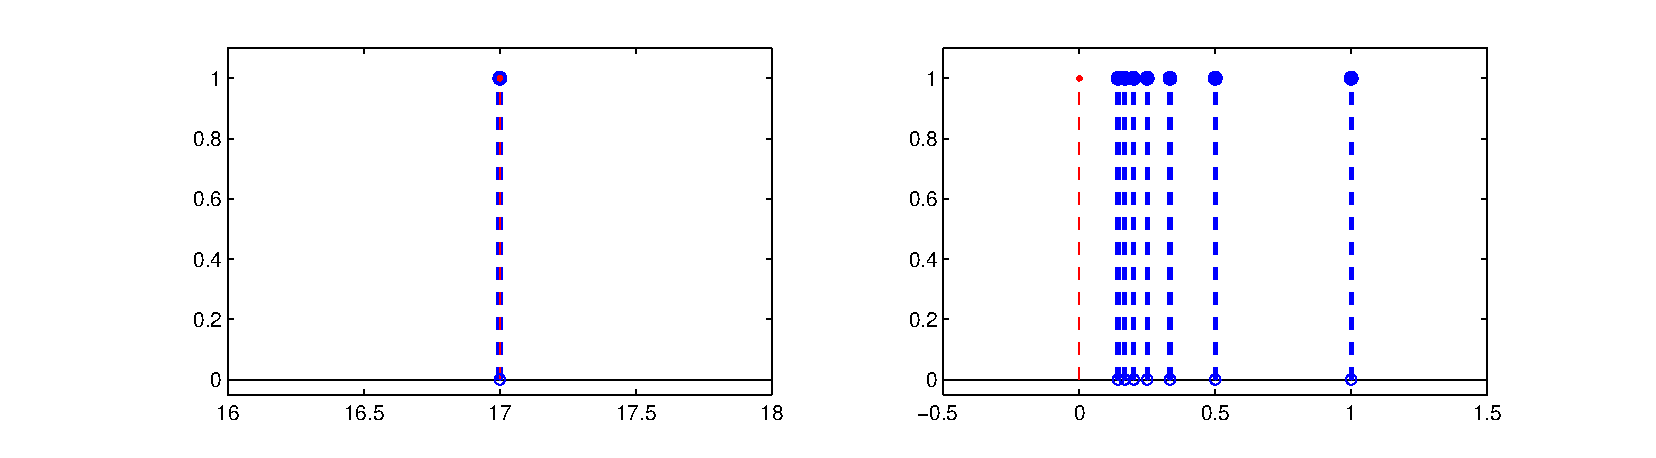
\includegraphics[width=6.5in]{figures/SequenceOfPointMassRVS17And1Byi}}
\end{figure}

\begin{classwork}[Convergence of $X_i \sim \normal(0,1/i)$]\label{CW:Normal01bynConvToPointMass0}
Suppose you are given an independent sequence of RVs $\{X_i \}_{i=1}^n$, where $X_i \sim \normal(0,1/i)$.  How would you talk about the convergence of $X_n \sim \normal(0,1/n)$ as $n$ approaches $\infty$ ?  Take a look at \hyperref[F:PlotNormal01bynConvToPointMass0]{Figure \ref*{F:PlotNormal01bynConvToPointMass0}} for insight.  The probability mass of $X_n$ increasingly concentrates about $0$ as $n$ approaches $\infty$ and the variance $1/n$ approaches $0$, as depicted in \hyperref[F:PlotNormal01bynConvToPointMass0]{Figure \ref*{F:PlotNormal01bynConvToPointMass0}}.  Based on this observation, can we expect $\lim_{n \rightarrow \infty} X_n = X$, where the limiting RV $X \sim \pointmass(0)$ ?

The answer is {\bf no}.  This is because $\p(X_n=X)=0$ for any $n$, since $X \sim \pointmass(0)$ is a discrete RV with exactly one outcome $0$ and $X_n \sim \normal(0,1/n)$ is a continuous RV for every $n$, however large.  In other words, a continuous RV, such as $X_n$, has $0$ probability of realizing any single real number in its support, such as $0$.    
\begin{figure}[htpb]
\caption{Distribution functions of several $\normal(\mu,\sigma^2)$ RVs for $\sigma^2 = 1,\frac{1}{10},\frac{1}{100},\frac{1}{1000}$.\label{F:PlotNormal01bynConvToPointMass0}}
\centering   \makebox{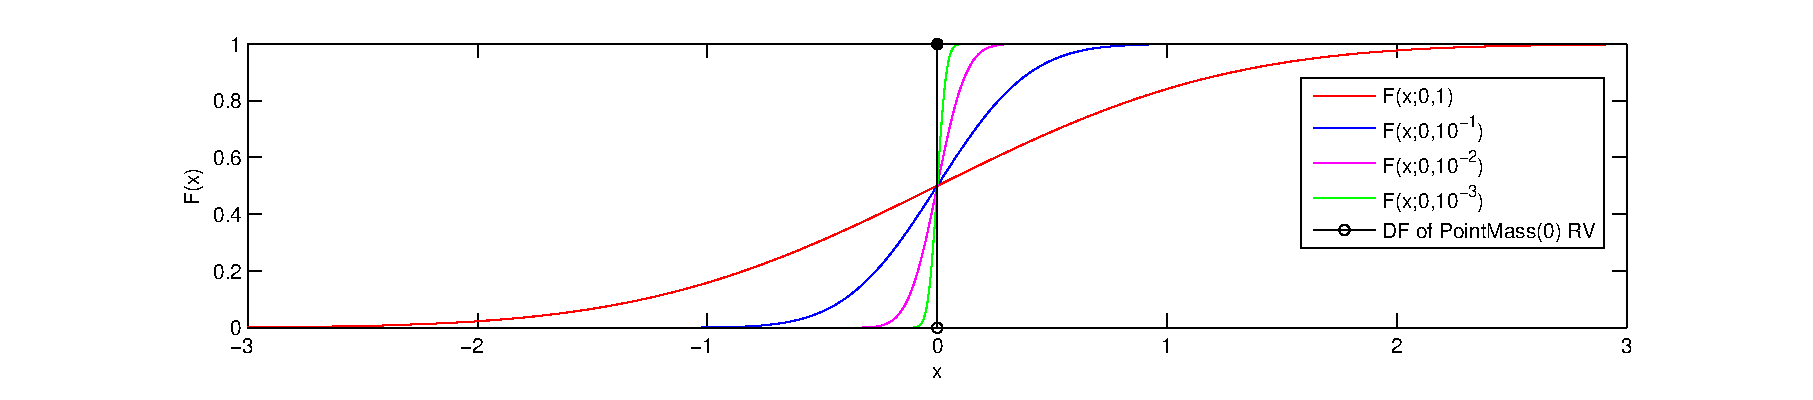
\includegraphics[width=6.5in]{figures/PlotNormal01bynConvToPointMass0}}
\end{figure}
\end{classwork}

Thus, we need more sophisticated notions of convergence for sequences of RVs.  Two such notions are formalized next as they are minimal prerequisites for a clear understanding of two basic propositions in Statistics :
\begin{enumerate} 
\item Law of Large Numbers,
\item Central Limit Theorem,
%\item Gilvenko-Cantelli Theorem.
\end{enumerate}

\begin{definition}[Convergence in Distribution (or Weakly, or in Law)]\label{D:ConvInDist}
Let $X_1,X_2,\ldots,$ be a sequence of RVs and let $X$ be another RV.  Let $F_n$ denote the DF of $X_n$ and $F$ denote the DF of $X$.  The we say that $X_n$ converges to $X$ in distribution, and write:
\[
X_n \rightsquigarrow X
\]
if for any real number $t$ at which $F$ is continuous,
\[
\lim_{n \rightarrow \infty} F_n(t) = F(t) \qquad \text{[in the sense of \hyperref[D:LimitofRealFunction]{Definition \ref*{D:LimitofRealFunction}}].}
\]
The above limit, by \eqref{E:DF} in our \hyperref[D:DF]{Definition \ref*{D:DF}} of a DF, can be equivalently expressed as follows: 
\begin{eqnarray}
& & \lim_{n \rightarrow \infty} \p( \ \{\omega: X_n(\omega) \leq  t \} \ )= 
\p( \ \{\omega: X(\omega) \leq  t \} \ ), \notag \\
&\text{i.e.~} & \p( \ \{\omega: X_n(\omega) \leq t \} \ ) \rightarrow \p( \ \{\omega: X(\omega) \leq  t \} \ ), \quad \text{as} \quad n \rightarrow \infty \notag \ .
\end{eqnarray}
\end{definition}

Let us revisit the problem of convergence in \hyperref[CW:Normal01bynConvToPointMass0]{Classwork \ref*{CW:Normal01bynConvToPointMass0}} armed with our new notions of convergence.
\begin{example}[Convergence in distribution]\label{EX:Normal01bynConvinDistToPointMass0}
Suppose you are given an independent sequence of RVs $\{X_i \}_{i=1}^n$, where $X_i \sim \normal(0,1/i)$ with DF $F_n$ and let $X \sim \pointmass(0)$ with DF $F$.  We can formalize our observation in \hyperref[CW:Normal01bynConvToPointMass0]{Classwork \ref*{CW:Normal01bynConvToPointMass0}} that $X_n$ is concentrating about $0$ as $n \to \infty$ by the statement:
\[
\text{$X_n$ is converging in distribution to $X$, ie,} \qquad X_n \rightsquigarrow X \ .
\]
{\scriptsize
\begin{proof}
To check that the above statement is true we need to verify that the definition of convergence in distribution is satisfied for our sequence of RVs $X_1,X_2,\ldots$ and the limiting RV $X$.  Thus, we need to verify that for any continuity point $t$ of the $\pointmass(0)$ DF $F$, $\lim_{n \to \infty} F_n(t)=F(t)$.  First note that 
\[
X_n \sim \normal(0,1/n) \implies Z := \sqrt{n} X_n \sim \normal(0,1) \ ,
\]
and thus
\[
F_n(t) = \p(X_n < t) = \p(\sqrt{n} X_n < \sqrt{n} t) = \p(Z < \sqrt{n} t) \ .
\]
The only discontinuous point of $F$ is $0$ where $F$ jump from $0$ to $1$.  

When $t < 0$, $F(t)$, being the constant $0$ function over the interval $(-\infty,0)$, is continuous at $t$.  Since $\sqrt{n} t \to -\infty$, as $n \to \infty$,
\[
\lim_{n \to \infty} F_n(t)  = \lim_{n \to \infty} \p(Z < \sqrt{n} t) = 0 = F(t) \ .
\]
And, when $t >0$, $F(t)$, being the constant $1$ function over the interval $(0,\infty)$, is again continuous at $t$.  Since $\sqrt{n} t \to \infty$, as $n \to \infty$,
\[
\lim_{n \to \infty} F_n(t)  = \lim_{n \to \infty} \p(Z < \sqrt{n} t) = 1 = F(t) \ .
\]
Thus, we have proved that $X_n \rightsquigarrow X$ by verifying that for any $t$ at which the $\pointmass(0)$ DF $F$ is continuous, we also have the desired equality: $\lim_{n \to \infty} F_n(t)=F(t)$.
\end{proof}
However, note that 
\[
F_n(0)=\frac{1}{2} \neq F(0)=1 \ ,
\]
and so convergence fails at $0$, i.e.~$\lim_{n \to \infty}F_n(t) \neq F(t)$ at $t=0$.  But, $t=0$ is not a continuity point of $F$ and the definition of convergence in distribution only requires the convergence to hold at continuity points of $F$.
}
\end{example}

Since $F(x) = \p(X \leq x)$, convergence in distribution means that the probability for $X_n$ to be in a given range is approximately equal to the probability that the value of the limiting RV $X$ is in that range, provided $n$ is sufficiently large. 

For a discrete sequence of RVs $X_n$`n to converge in distribution to another discrete RV $X$ taking values in $\mathbb{Z}_+ = \{0,1,2,\ldots\}$, it is sufficient to show that $\lim_{n \to \infty}\p(X_n = x) = \p(X=x)$ for each $x \in \mathbb{Z_+}$.  
We will use this fact to prove why we can approximate $\binomial$ RVs by a $\poisson$ under some limiting conditions.

\subsubsection{$\binomial(n,\lambda/n)$ convergence in distribution to $\poisson(\lambda)$ as $n \to \infty$, $\theta=\lambda/n \to 0$}
In several situations, as we saw already, it becomes cumbersome to model the events using the $\binomial(n,\theta)$ RV, especially when when the parameter $\theta \propto 1/n$ and the events become rare.  
However, for some real parameter $\lambda>0$, the $\binomial(n,\lambda/n)$ RV with probability of the number of successes in $n$ trials, with per-trial success probability $\lambda/n$, approaches the Poisson distribution with expectation $\lambda$, as $n$ approaches $\infty$ (actually, it converges in distribution).  
The $\poisson(\lambda)$ RV is much simpler to work with than the combinatorially laden $\binomial(n,\theta=\lambda/n)$ RV.  We sketch the details of this next.

Let $X_n \sim \binomial(n,\theta=\lambda/n)$ and $Y \sim \poisson(\lambda)$ and let $\lambda=n\theta$ remain constant as  $n \to \infty$, $\theta \to 0$.  
We need to show that $\lim_{n \to \infty} \p(X_n=x) = \p(Y=x) = e^{-\lambda}\lambda^x/x!$ for any $x \in \{0,1,2,3,\ldots,n\}$. 
%{\scriptsize
\begin{eqnarray}
\p(X=x)
&=&
\binom{n}{x} \left( \frac{\lambda}{n} \right)^x \left( 1- \frac{\lambda}{n} \right)^{n-x} \notag \\
&=& \frac{n(n-1)(n-2)\cdots(n-x+1)}{x(x-1)(x-2)\cdots (2)(1)}
\left( \frac{\lambda^x}{n^x} \right)
\left( 1- \frac{\lambda}{n} \right)^n
\left( 1- \frac{\lambda}{n} \right)^{-x} \notag \\
&=&
\overbrace{\left( \frac{n}{n} \right) \left( \frac{n-1}{n} \right) \left( \frac{n-2}{n} \right) \cdots \left( \frac{n-x+1}{n} \right)}
\overbrace{\left( \frac{\lambda^x}{x!} \right)}
\underbrace{\left( 1- \frac{\lambda}{n} \right)^n}
\underbrace{\left( 1- \frac{\lambda}{n} \right)^{-x}}  \notag \\
\end{eqnarray}

As $n \to \infty$, the expression below the first overbrace $\to 1$, while that below the second overbrace, being independent of $n$ remains the same.  By the elementary examples of limits
%\remove{
\ref*{EX:LimitExpofLambda} and \ref*{EX:Limit1MinusLambdaOverNToMinusK}%}
, as $n \to \infty$, the expression over the first underbrace approaches $e^{-\lambda}$ while that over the second underbrace approaches $1$.  Finally, we get the desired limit:

\[
\lim_{n \to \infty} \p(X=x)
= \frac{ e^{-\lambda} \lambda^x}{x!}  \ .
\]
%}

\begin{rem}[Scheff\'e's Theorem]
Convergence in distribution does not in general imply that the sequence of corresponsing probability density functions will also converge. 
Consider for example RV $X_n$ with density $\BB{1}_{(0,1)}(x)(1-\cos(2\pi n x))$. 
These RVs converge in distribution to $X \sim \uniform(0,1)$, but their densities do not converge at all.

However, according to {\bf Scheff\'e's Theorem} convergence of the probability density function implies convergence in distribution.
\end{rem}

The second notion of convergence of RVs is convergence in probability.

\begin{definition}[Convergence in Probability]\label{D:ConvInProb}
Let $X_1,X_2,\ldots,$ be a sequence of RVs and let $X$ be another RV.  Let $F_n$ denote the DF of $X_n$ and $F$ denote the DF of $X$.  The we say that $X_n$ converges to $X$ in probability, and write:
\[
X_n \overset{P}{\longrightarrow} X
\]
if for every real number $\epsilon > 0$,
\[
\lim_{n \rightarrow \infty} \p(|X_n-X|> \epsilon) = 0 \qquad \text{[in the sense of \hyperref[D:LimitofRealFunction]{Definition \ref*{D:LimitofRealFunction}}].}
\]
Once again, the above limit, by \eqref{E:ProbOfRV} in our \hyperref[D:RV]{Definition \ref*{D:RV}} of a RV, can be equivalently expressed as follows: 
\[
\lim_{n \rightarrow \infty} \p( \ \{\omega: |X_n(\omega) - X(\omega)| > \epsilon\} \ )=0, \qquad \text{ie,} \qquad \p( \ \{\omega: |X_n(\omega) - X(\omega)| > \epsilon\} \ ) \rightarrow 0, \quad \text{as} \quad n \rightarrow \infty \ .
\]
\end{definition}
 
For the same sequence of RVs in  \hyperref[CW:Normal01bynConvToPointMass0]{Classwork \ref*{CW:Normal01bynConvToPointMass0}} and \hyperref[EX:Normal01bynConvinDistToPointMass0]{Example \ref*{EX:Normal01bynConvinDistToPointMass0}} we are tempted to ask whether $X_n \sim \normal(0,1/n)$ converges in probability to $X \sim \pointmass(0)$, i.e.~whether $X_n \overset{P}{\longrightarrow} X$.  We need some elementary inequalities in Probability to help us answer this question.  We visit these inequalities next.


\begin{prop}[Markov's Inequality]
Let $(\Omega,\C{F},P)$ be a probability triple and let $X=X(\omega)$ be a non-negative RV.  Then,
\begin{equation}\label{E:MarkovNeq}
\p(X \geq \epsilon) \leq \frac{\e(X)}{\epsilon}, \qquad \text{for any} \quad \epsilon > 0 \ .
\end{equation}
{\scriptsize
\begin{proof}
\begin{eqnarray}
X &=& X \BB{1}_{ \{y: y \geq \epsilon \} } (x) + X \BB{1}_{ \{y: y < \epsilon \} } (x) \notag \\
&\geq& X \BB{1}_{ \{y: y \geq \epsilon \} } (x) \notag \\
&\geq& \epsilon  \BB{1}_{ \{y: y \geq \epsilon \} } (x) \notag \\
\end{eqnarray}
Finally, taking expectations on both sides of the above inequality and then using the fact that the expectation of an indicator function of an event is simply the probability of that event \eqref{E:ExpectationofIndicator}, we get the desired result:
\[
\e(X) \geq \epsilon \e( \BB{1}_{ \{y: y \geq \epsilon \} } (x)) = \epsilon \p(X \geq \epsilon) \ .
\]
\end{proof}
}
\end{prop}
Let us look at some immediate consequences of Markov's inequality.
\begin{prop}[Chebychev's Inequality]
For {\bf any} RV $X$ and any $\epsilon > 0$,
\begin{eqnarray}
\p(|X| > \epsilon) &\leq& \frac{\e(|X|)}{\epsilon} \label{E:ChebychevNeq1} \\
\p(|X| > \epsilon) = \p(X^2 \geq \epsilon^2) &\leq& \frac{\e(X^2)}{\epsilon^2} \label{E:ChebychevNeq2} \\
\p(|X-\e(X)| \geq \epsilon) = \p((X-\e(X))^2 \geq \epsilon^2) &\leq& \frac{\e(X-\e(X))^2}{\epsilon^2}  = \frac{\V(X)}{\epsilon^2}  \label{E:ChebychevNeq3} 
\end{eqnarray}
{\scriptsize
\begin{proof}
All three forms of Chebychev's inequality are mere corollaries (careful reapplications) of Markov's inequality.
\end{proof}
}
\end{prop}

Armed with Markov's inequality we next enquire the convergence in probability for the sequence of RVs in \hyperref[CW:Normal01bynConvToPointMass0]{Classwork \ref*{CW:Normal01bynConvToPointMass0}} and \hyperref[EX:Normal01bynConvinDistToPointMass0]{Example \ref*{EX:Normal01bynConvinDistToPointMass0}}.

\begin{example}[Convergence in probability]\label{EX:Normal01bynConvinProbToPointMass0}
Does the the sequence of RVs $\{X_n\}_{n=1}^{\infty}$, where $X_n \sim \normal(0,1/n)$, converge in probability to $X \sim \pointmass(0)$, i.e.~does $X_n \overset{P}{\longrightarrow} X$ ?

To find out if $X_n \overset{P}{\longrightarrow} X$, we need to show that for any $\epsilon >0$, $\lim_{n \to \infty} \p(|X_n-X|>\epsilon)=0$.

Let $\epsilon$ be any real number greater than $0$, then
\begin{eqnarray}
\p(|X_n|>\epsilon) &=& \p(|X_n|^2 > \epsilon^2) \notag \\
&\leq& \frac{\e(X_n^2)}{\epsilon^2} \qquad \text{[by Markov's Inequality \eqref{E:MarkovNeq}]} \notag \\
&=& \frac{\frac{1}{n}}{\epsilon^2} \to 0, \quad \text{as} \quad n \to \infty \qquad \text{[in the sense of \hyperref[D:LimitofRealFunction]{Definition \ref*{D:LimitofRealFunction}}].} \notag
\end{eqnarray}
Hence, we have shown that for any $\epsilon >0$, $\lim_{n \to \infty} \p(|X_n-X|>\epsilon)=0$ and therefore by \hyperref[D:ConvInProb]{Definition \ref*{D:ConvInProb}}, $X_n \overset{P}{\longrightarrow} X$ or $X_n \overset{P}{\longrightarrow} 0$.  

{\scriptsize
{\bf Convention:} When $X$ has a $\pointmass(\theta)$ distribution and $X_n \overset{P}{\longrightarrow} X$, we simply write $X_n \overset{P}{\longrightarrow} \theta$.
}
\end{example}

\begin{definition}[Convergence Almost Surely (or with Probability $1$)]
To say that the sequence of RVs $\{X_n\}_{n=1}^{\infty}$ converges almost surely (or with probability $1$ or strongly) towards another RV $X$ on the same probability space $(\Omega,\mathcal{F},\p)$, as denoted by
\[
X_n \overset{a.s.}{\to} X
\]
means that
\[
\p \left( \{ \lim_{n \to \infty} X_n = X \} \right) = 1 \quad \iff \quad \p \left( \{\omega \in \Omega : \lim_{n \to \infty} X_n(\omega) = X(\omega)\} \right) = 1.
\]
This means that the values of $X_n$ approach the value of $X$, in the sense that events for which $X_n$ does not converge to $X$ have probability $0$.
\end{definition}

Other notions of convergence are termed sure convergence or pointwise convergence, such as convergence in mean. 
But the above three types of convergence are elementary. % and enough to appreciate the subtle issues with convergence of random variables.

\begin{Exercise}[title={Example Classwork},label={xExample}]
After reading Sec.~\ref{S:ConvOfRVs} up to now, think carefully about what you need to be able to show that $Z_n := 1/\sqrt{n}\sum_{i=1}^n X_i$ converges in distribution to the $\normal(0,1/3)$ RV, where $X_i \overset{IID}{\sim} \uniform(-1,1)$. {Hint: Characteristic functions}
%\ExePart
%\Question
%\subQuestion Show that...
%\subQuestion In this question...
%\subsubQuestion Show that...
%\subsubQuestion Conclude...
%\subQuestion Conclude.
%\Question Show that if $b > 1$...
%\ExePart
%\Question What happens to if $b=1$?
\end{Exercise}

\begin{prop}[Weak Law of Large Numbers (WLLN)]
If we are given a sequence if independent and identically distributed RVs, $X_1,X_2,\ldots \overset{\IID}{\sim} X_1$ and if $\e(X_1)$ exists, as per \eqref{E:ExpectationExists}, then the sample mean $\overline{X}_n$ converges in probability to the expectation of any one of the IID RVs, say $\e(X_1)$ by convention.  More formally, we write:
\[
\text{If} \quad X_1,X_2,\ldots \overset{\IID}{\sim} X_1 \ \text{and if } \ \e(X_1) \ \text{exists, then } \ \overline{X}_n \overset{P}{\longrightarrow} \e(X_1) \ .
\]
{\scriptsize
\begin{proof}
For simplicity, we will prove a slightly weaker result by assuming finite variance of $X_1$.  Suppose $\V(X_1) < \infty$, then:
\begin{eqnarray}
\p(| \overline{X}_n - \e(\overline{X}_n) | \geq \epsilon)
&=& \frac{\V(\overline{X}_n)}{\epsilon^2} \qquad \text{{\scriptsize [by applying Chebychev's inequality \eqref{E:ChebychevNeq3} to the RV $\overline{X}_n$]}} \notag \\
&=& \frac{\frac{1}{n}\V(X_1)}{\epsilon^2} \qquad \text{{\scriptsize [by the IID assumption of $X_1,X_2,\ldots$ we can apply \eqref{E:VarOfSampleMeanOfIIDSeq}]}} \notag 
\end{eqnarray}
Therefore, for any given $\epsilon>0$,
\begin{eqnarray}
\p(| \overline{X}_n - \e(X_1) | \geq \epsilon)
&=&  \p(| \overline{X}_n - \e(\overline{X}_n) | \geq \epsilon) \qquad \text{{\scriptsize [by the IID assumption of $X_1,X_2,\ldots$,  $\e(\overline{X}_n)=\e(X_1)$, as per \eqref{E:ExpOfSampleMeanOfIDSeq}]}} \notag \\
&=&  \frac{\frac{1}{n}\V(X_1)}{\epsilon^2} \to 0, \quad \text{as} \quad n \to \infty \ , \notag
\end{eqnarray}
or equivalently, $\lim_{n \to \infty} \p(| \overline{X}_n - \e(X_1) | \geq \epsilon) = 0$.  And the last statement is the definition of the claim made by the weak law of large numbers (WLLN), namely that $\overline{X}_n \overset{P}{\longrightarrow} \e(X_1)$ .
\end{proof}
}
{\bf Heuristic Interpretation of WLLN:}  
The distribution of the sample mean RV $\overline{X}_n$ obtained from an independent and identically distributed sequence of RVs $X_1,X_2,\ldots$ {\scriptsize [i.e.~all the RVs $X_i$'s are independent of one another and have the same distribution function, and thereby the same expectation, variance and higher moments]}, concentrates around the expectation of any one of the RVs in the sequence, say that of the first one $\e(X_1)$ {\scriptsize [without loss of generality]}, as $n$ approaches infinity.  See Figure~\ref{F:RunningMeansFairDieFairCoinUnif01Exp1By10} for examples of 20 replicates of the sample mean of IID sequences from four RVs.  All the sample mean trajectories converge to the corresponding population mean. 

\begin{figure}[htpb]
\caption{Sample mean $\ol{X}_n$ as a function of sample size $n$ for 20 replications from independent realizations of a fair die (blue), fair coin (magenta), $\uniform(0,30)$ RV (green) and $\exponential(0.1)$ RV (red) with population means $(1+2+3+4+5+6)/6=21/6=3.5$, $(0+1)/2=0.5$, $(30-0)/2=15$ and $1/0.1=10$, respectively.\label{F:RunningMeansFairDieFairCoinUnif01Exp1By10}}
\centering   \makebox{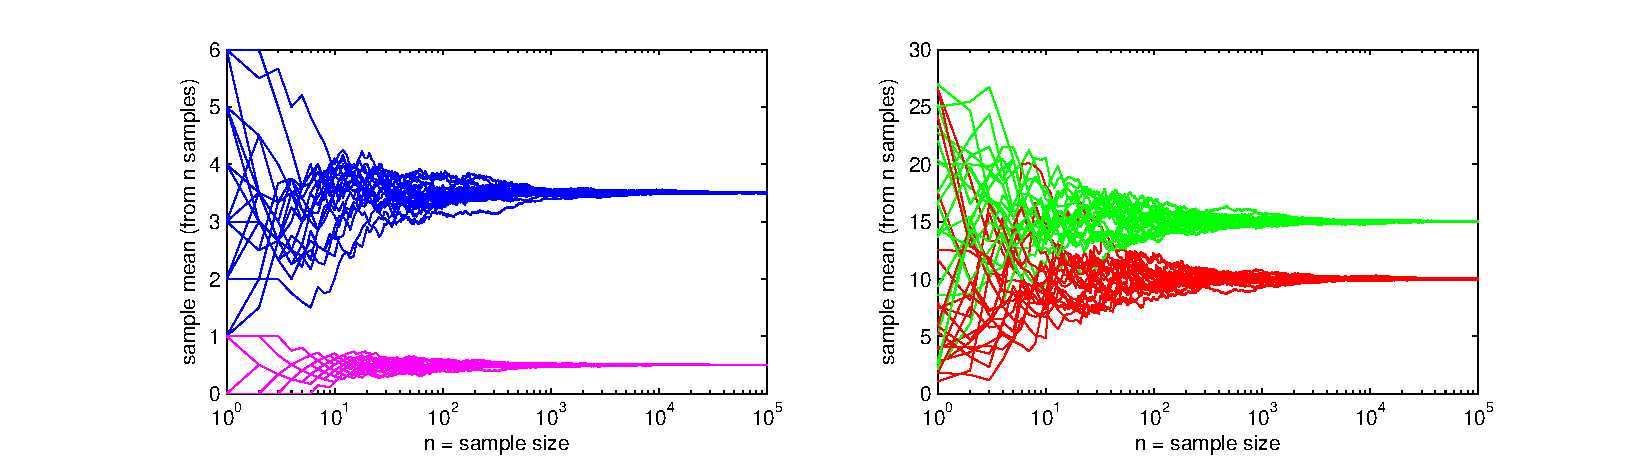
\includegraphics[width=6.5in]{figures/RunningMeansFairDieFairCoinUnif01Exp1By10}}
\end{figure}

\end{prop}
\begin{example}[Bernoulli WLLN and Galton's Quincunx]
We can appreciate the WLLN for $\overline{X}_n = n^{-1} S_n = \sum_{i=1}^{n} X_i$, where $X_1,X_2,\ldots,X_n \overset{\IID}{\sim} Bernoulli(p)$ using the paths of balls dropped into a device built by Galton called the Quincunx.
\end{example}



\subsubsection{Properties of Convergence of RVs}

We will merely state some properties (without proofs as they are advanced for this course) and relations between the three notions of convergence with some examples to better appreciate the subtleties among them.

%L\'evy's Continuity Theorem on CFs before proof og CLT via CFs

Now that we have been introduced to three notions of convergence for sequences of RVs we can begin to appreciate the  construction of limiting random variables from existing ones. % We will see a limiting sum of $n$ independent $\bernoulli(\theta)$ RVs as $n \to \infty$ and $\theta \to 0$ such that $n \theta = \lambda$. %  statements of the basic limit theorems of Statistics.  
But first we need some analytic tools.

%But first we formally define a statistic.


\begin{prop}[Central Limit Theorem (CLT)]
Let $X_1,X_2,\ldots \overset{\IID}{\sim} X_1$ and suppose $\e(X_1)$ and $\V(X_1)$ exists, then 
{\small
\begin{eqnarray}
%1
\overline{X}_n = \frac{1}{n} \sum_{i=1}^n X_i 
& \rightsquigarrow & 
X \sim \normal \left( \e(X_1),\frac{\V(X_1)}{n}  \right) \ , \\
%2
\overline{X}_n -\e(X_1) 
& \rightsquigarrow & 
X-\e(X_1) \sim \normal \left( 0,\frac{\V(X_1)}{n}  \right) \ , \\
%3
\sqrt{n} \left( \overline{X}_n -\e(X_1) \right)
& \rightsquigarrow & 
\sqrt{n} \left( X-\e(X_1) \right) \sim \normal \left( 0,\V(X_1)  \right) \ , \\
%4
Z_n :=  \frac{\overline{X}_n-\e(\overline{X}_n)}{\sqrt{\V(\overline{X}_n)}} 
= \frac{\sqrt{n} \left( \overline{X}_n -\e(X_1) \right)}{\sqrt{\V(X_1)}}
& \rightsquigarrow & 
Z  \sim \normal \left( 0,1  \right) \ , \\
%5
\lim_{n \to \infty} P\left( \frac{\overline{X}_n-\e(\overline{X}_n)}{\sqrt{\V(\overline{X}_n)}}  \leq z \right)
= \lim_{n \to \infty} \p(Z_n \leq z)
&=&
\Phi(z) := \int_{- \infty}^z \left( \frac{1}{\sqrt{2 \pi}} \ \exp \left( \frac{-x^2}{2} \right) \right) dx \ .
\end{eqnarray}
}
Thus, for sufficiently large $n$ (say $n>30$) we can make the following approximation:
\begin{equation}\label{E:CLTApprox}
P\left( \frac{\overline{X}_n-\e(\overline{X}_n)}{\sqrt{\V(\overline{X}_n)}}  \leq z \right) 
\approxeq 
\p(Z \leq z)
=
\Phi(z) := \int_{- \infty}^z \left( \frac{1}{\sqrt{2 \pi}} \ \exp \left( \frac{-x^2}{2} \right) \right) dx \ .
\end{equation}
{\scriptsize
\begin{proof}
See any intermediate to advanced undergraduate text in Probability.  Start from the index looking for ``Central Limit Theorem'' to find the page number for the proof \ldots .
\end{proof}
}
{\bf Heuristic Interpretation of CLT:}  Probability statements about the sample mean RV $\overline{X}_n$ can be approximated using a Normal distribution. 
\end{prop}
Here is a simulation showing CLT in action.
\begin{VrbM}
>> % a demonstration of Central Limit Theorem --
>> % the sample mean of a sequence of n IID Exponential(lambda) RVs 
>> % itself a Gaussian(1/lambda,lambda/n) RV
>> lambda=0.1; Reps=10000; n=10; hist(sum(-1/lambda * log(rand(n,Reps)))/n)
>> lambda=0.1; Reps=10000; n=100; hist(sum(-1/lambda * log(rand(n,Reps)))/n,20)
>> lambda=0.1; Reps=10000; n=1000; hist(sum(-1/lambda * log(rand(n,Reps)))/n,20)
\end{VrbM}

Let us look at an example that makes use of the CLT next.
\begin{example}[Errors in computer code (Wasserman03, p.~78)]\label{EX:CLTPoisson}
Suppose the collection of RVs $X_1,X_2, \ldots, X_n$ model the number of errors in $n$ computer programs named $1,2,\ldots,n$, respectively.  Suppose that the RV $X_i$ modeling the number of errors in the $i$-th program is the $Poisson(\lambda=5)$ for any $i=1,2,\ldots,n$.  Further suppose that they are independently distributed.  Succinctly, we suppose that 
\[
X_1,X_2,\ldots,X_n \overset{\IID}{\sim} \poisson(\lambda=5) \ . 
\]
Suppose we have $n=125$ programs and want to make a probability statement about $\overline{X}_n$ which is the average error per program out of these $125$ programs.  Since $\e(X_i) = \lambda=5$ and $\V(X_i)=\lambda=5$, we may want to know how often our sample mean $\overline{X}_{125}$ differs from the expectation of $5$ errors per program.  Using the CLT we can approximate $\p(\overline{X}_n < 5.5)$, for instance, as follows:
\begin{eqnarray}
\p(\overline{X}_n < 5.5) 
&=& P \left( \frac{\sqrt{n}(\overline{X}_n - \e(X_1))}{\sqrt{\V(X_1)}} < \frac{\sqrt{n}(5.5-\e(X_1))}{\sqrt{\V(X_1)}} \right) \notag \\
&\approxeq& P \left( Z < \frac{\sqrt{n}(5.5-\lambda)}{\sqrt{\lambda}} \right) \qquad \text{{\scriptsize [by \eqref{E:CLTApprox}, and $\e(X_1)=\V(X_1)=\lambda$]}} \notag \\
&=& P \left( Z < \frac{\sqrt{125}(5.5-5)}{\sqrt{5}} \right) \qquad \text{{\scriptsize [Since, $\lambda=5$ and $n=125$ in this Example]}} \notag \\
&=& \p(Z \leq 2.5) = \Phi(2.5) =  \int_{- \infty}^{2.5} \left( \frac{1}{\sqrt{2 \pi}} \ \exp \left( \frac{-x^2}{2} \right) \right) dx \approxeq 0.993790334674224 \ . \notag
\end{eqnarray}
The last number above needed the following:
\begin{labwork}[Numerical approximation of $\Phi(2.5)$]
The numerical approximation of $\Phi(2.5)$ was obtained via the following call to our $\erf$-based {\tt NormalCdf} function. % from \ref*{Mf: NormalCdfPdf}. MATLABback
\begin{VrbM}
>> format long
>> disp(NormalCdf(2.5,0,1))
   0.993790334674224
\end{VrbM}
\end{labwork}
\end{example}
The CLT says that if $X_1,X_2,\ldots \overset{\IID}{\sim} X_1$, then $Z_n := \sqrt{n}(\overline{X}_n-\e(X_1))/\sqrt{\V(X_1)}$ is approximately distributed as $\normal(0,1)$.  In \hyperref[EX:CLTPoisson]{Example \ref*{EX:CLTPoisson}}, we knew $\sqrt{\V(X_1)}$.   However, in general, we may not know $\sqrt{\V(X_1)}$.  The next proposition says that we may estimate $\sqrt{\V(X_1)}$ using the sample standard deviation $S_n$ of $X_1,X_2,\ldots,X_n$, according to \eqref{E:SampleStdDevRV}, and still make probability statements about the sample mean $\overline{X}_n$ using a Normal distribution.
\begin{prop}[CLT based on Sample Variance]
Let $X_1,X_2,\ldots \overset{\IID}{\sim} X_1$ and suppose $\e(X_1)$ and $\V(X_1)$ exists, then
\begin{equation}\label{E:CLTApproxSn}
\frac{\sqrt{n} \left( \overline{X}_n - \e(X_1) \right)}{S_n} \rightsquigarrow \normal(0,1) \ .
\end{equation}
\end{prop}

We will use \eqref{E:CLTApproxSn} for statistical estimation in the sequel.

%The next proposition is often referred to as the fundamental theorem of statistics and is at the heart of non-parametric inference, empirical processes, and computationally-intensive bootstrap techniques.
%\begin{prop}[Gilvenko-Cantelli Theorem]\label{P:Gilvenko-Cantelli}
%Let $X_1,X_2,\ldots,X_n \overset{\IID}{\sim} F$.  Then,
%\[
%\sup_x { | \widehat{F}_n(x) - F(x) | } \overset{P}{\longrightarrow} 0 \ .
%\]
%{\scriptsize
%\begin{proof}
%Proof to be seen in STAT 318 or another advanced Statistics course.
%\end{proof}
%}
%\end{prop}
%{\bf Heuristic Interpretation of Gilvenko-Cantelli Theorem}:  As the sample size $n$ increases the empirical distribution function $\widehat{F}_n$ converges to the true DF $F$ in probability.

%\begin{figure}[htpb]
%\caption{Plots of ten distinct ECDFs $\widehat{F}_n$ based on $10$ sets of $n$ IID samples from $\uniform(0,1)$ RV $X$, as $n$ increases from $10$ to $100$ to $1000$.  The DF $F(x)=x$ over $[0,1]$ is shown in red.  The script of \hyperref[Mf:GilvenkoCantelliUnif01n10n100n100ECDFs]{Labwork \ref*{Mf:GilvenkoCantelliUnif01n10n100n100ECDFs}} was used to generate this plot.   \label{F:GilvenkoCantelliUnif01n10n100n100ECDFs}}
%\centering   \makebox{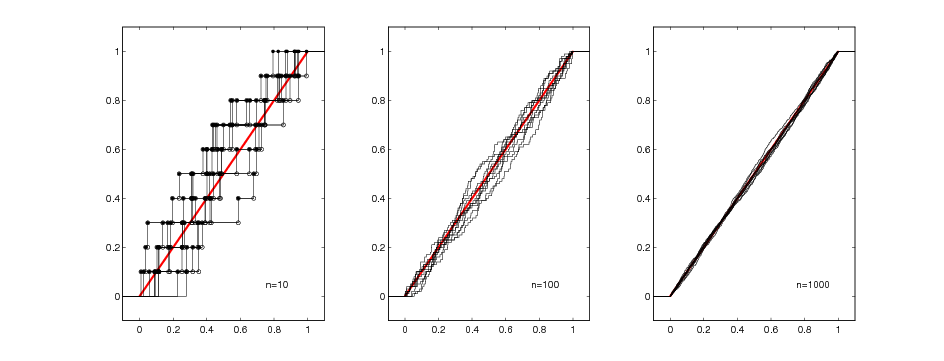
\includegraphics[width=7.0in]{figures/GilvenkoCantelliUnif01n10n100n100ECDFs}}
%\end{figure}

%\begin{prop}[The Dvoretzky-Kiefer-Wolfowitz (DKW) Inequality]
%Let $X_1,X_2,\ldots,X_n \overset{\IID}{\sim} F$.  Then, for any $\epsilon>0$,
%\begin{equation}\label{E:DKWNeq}
%P \left( \sup_x | \widehat{F}_n(x) - F(x) | > \epsilon  \right) \leq 2 \exp {(-2 n \epsilon^2)}
%\end{equation}
%\end{prop}
